\chapter{}

\section{Enunciado}

Analizar y probar gramáticas libres y dependientes del contexto con jFlap.

\section{Solución}

Vamos a trabajar primero con la siguiente gramática libre del contexto:

\begin{align*}
	G &= (V, T, P, S) : \\
	V &= \{S, A, B\} \\
	T &= \{a, b\} \\
	P &=
		\begin{cases}
		\begin{array}{ll}
			S \rightarrow aB & A \rightarrow bAA \\
			S \rightarrow bA & B \rightarrow b   \\
			A \rightarrow a  & B \rightarrow bS  \\
			A \rightarrow aS & B \rightarrow aBB \\
		\end{array}
 		\end{cases} \\
	S &= S
\end{align*}

La introducimos en jFlap:

\begin{figure}[h!]
\begin{center}
	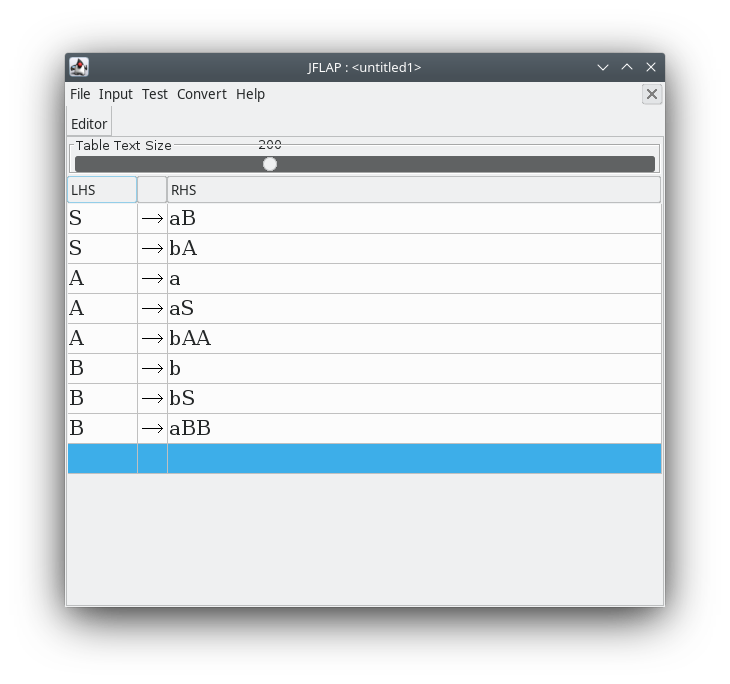
\includegraphics[scale=0.4]{Prácticas/jFlap - Gramática libre del contexto}
\end{center}
\caption{Introducción de la primera gramática en jFlap.}
\end{figure}

\pagebreak

Procedemos a ejecutarla:

\begin{figure}[h!]
\begin{center}
	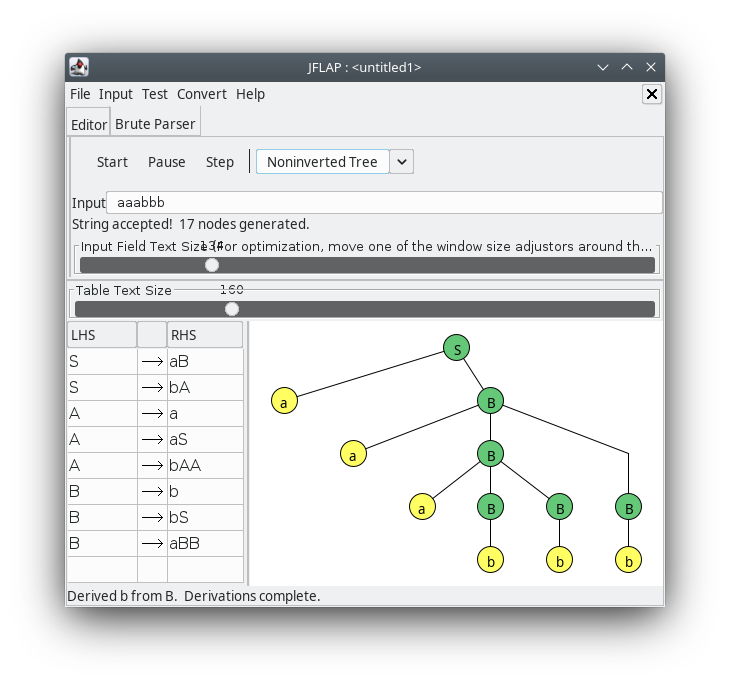
\includegraphics[scale=0.4]{Prácticas/jFlap - Gramática libre del contexto ejecución}
	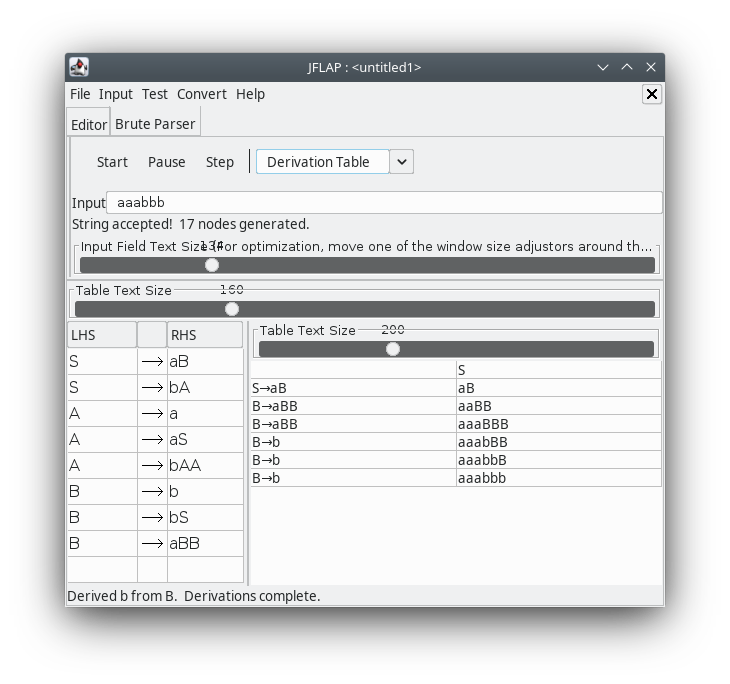
\includegraphics[scale=0.4]{Prácticas/jFlap - Gramática libre del contexto derivación}
\end{center}
\caption{Ejecución y tabla de derivación de la primera gramática en jFlap.}
\end{figure}

Vamos ahora a trabajar con la siguiente gramática dependiente del contexto:

\begin{align*}
	G &= (V, T, P, S) : \\
	V &= \{S, X, Y\} \\
	T &= \{a, b, c\} \\
	P &=
		\begin{cases}
		\begin{array}{ll}
			S \rightarrow abc   & bY \rightarrow Yb  \\
			S \rightarrow aXbc  & aY \rightarrow aaX \\
			Xb \rightarrow bX   & aY\rightarrow aa   \\
			Xc \rightarrow Ybcc &                    \\
		\end{array}
 		\end{cases} \\
	S &= S
\end{align*}

\pagebreak

La introducimos en jFlap:

\begin{figure}[h!]
\begin{center}
	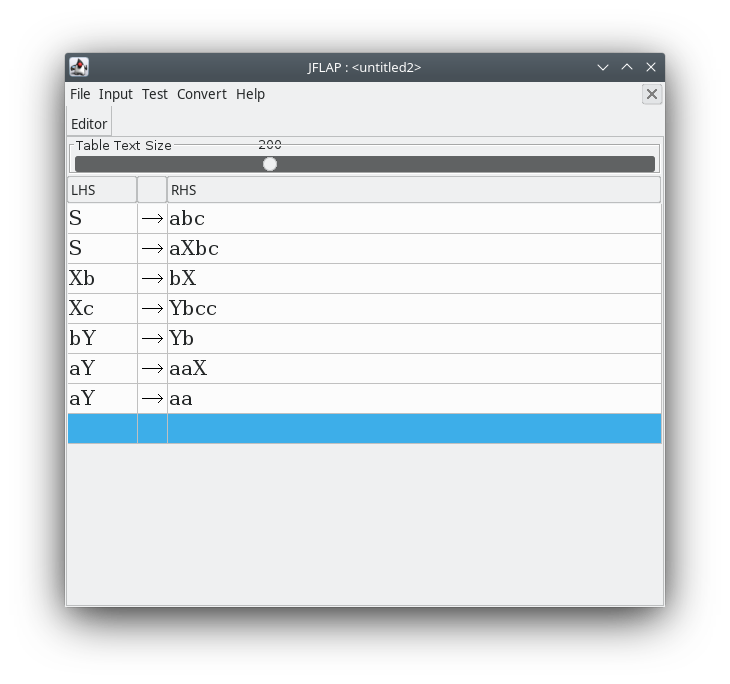
\includegraphics[scale=0.4]{Prácticas/jFlap - Gramática dependiente del contexto}
\end{center}
\caption{Introducción de la segunda gramática en jFlap.}
\end{figure}

Procedemos a ejecutarla:

\begin{figure}[h!]
\begin{center}
	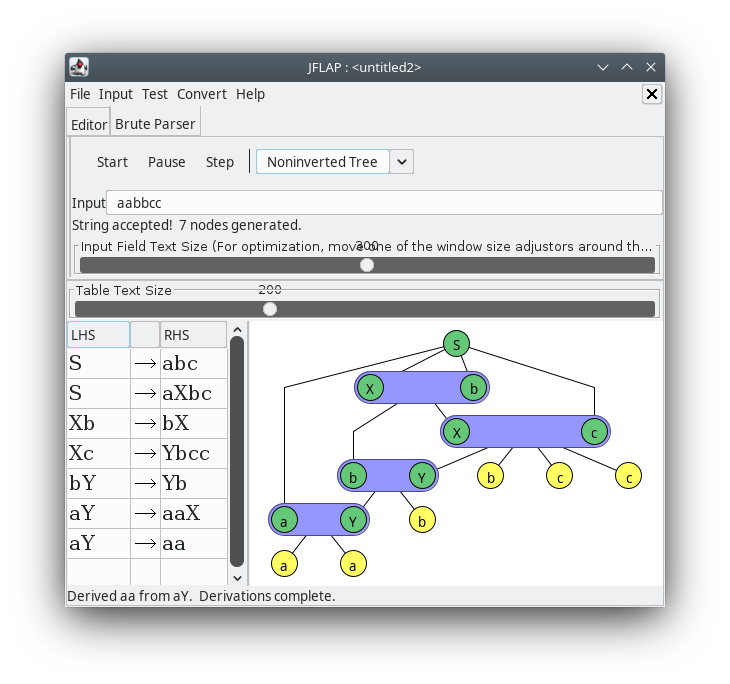
\includegraphics[scale=0.4]{Prácticas/jFlap - Gramática dependiente del contexto ejecución}
	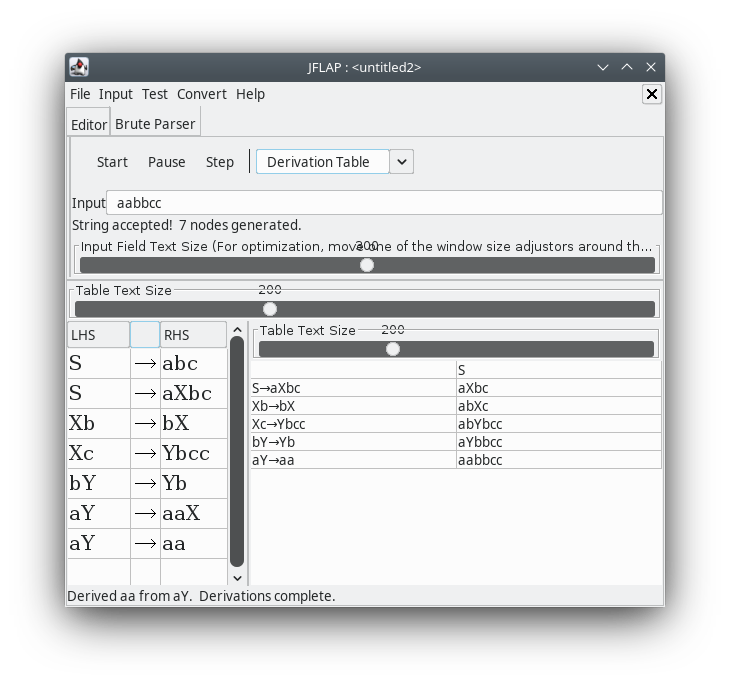
\includegraphics[scale=0.4]{Prácticas/jFlap - Gramática dependiente del contexto derivación}
\end{center}
\caption{Ejecución y tabla de derivación de la segunda gramática en jFlap.}
\end{figure}
